 \documentclass[12pt]{article}
 \usepackage{graphicx}
 \usepackage{multirow}
 \usepackage{amsmath}
 \usepackage{fullpage}
 \usepackage{times}
 \setlength\parindent{0pt}
 \setlength\parskip{12pt}

 \usepackage{bigstrut}

 \begin{document}

 {\sffamily
 \begin{tabular}{lll}
 \multirow{8}{1in}{\includegraphics[width=1in]{ach.png}} & &\\%\multirow{9}{1in}{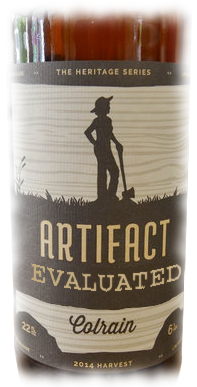
\includegraphics[width=1in]{eval.png}}\\
 & &\\
 & \large{\em CONFIDENTIAL COMMITTEE MATERIALS} &\\
 & &\\
 & \textbf{\LARGE{SIGBOVIK 2016 Artifact Evaluation}}& \\
 & &\\
 & \Large{Paper 12: Which ITG Stepcharts are Turniest?} & \\
 &\\
 \vspace{1em}\\
 \hline
 \end{tabular}}
 \vspace{2em}
 \thispagestyle{empty}


\textbf{Claim 1:}  \textit{LURR DURR}

\textbf{EVALUATION OF CLAIM:}
  The evaluation committee tripped repeatedly while attempting to
  evaluate this claim, leading to the loss of several perfectly good ``candles.'' The committee requests
  an instructional video on performing this maneuver, as well as a fresh 6-pack of Woodchuck.

  Though the committee does concede evaluating this claim would have been easier if we weren’t
  halfway through the 6-pack of Woodchuck when we started.

\textbf{Claim 2:}  \textit{Real-world tracks achieve 81.33\% of the theoretical maximum turniness.}

\textbf{EVALUATION OF CLAIM:}
  The evaluation committee has confirmed that .8133 * 2 = 1.6266 which is an
  appropriate rounding-down of the number 1.6267 that appears on the spreadsheet. We appreciate
  the author's willingness to round numbers in the least favorable a direction, a subject with which
  we understand systems researchers frequently struggle.

  However, the artifact submitted contains no actual stepcharts, let alone songs, and thus we have no
  way to evaluate whether this claim is actually true.

  We were about to reject your submission for this reason, but then a member of the committee
  discovered an algorithm for turning theoretical stepcharts into real stepcharts. Followed by the
  insight that 1.6266 \textless 2.0, we discovered that the author is indeed capable of producing such a
  stepchart upon request.

\textbf{Claim 3:}  \textit{The author is capable of multiplying various numbers by 10000.}

\textbf{EVALUATION OF CLAIM:}
  We diligently verified your multiplication of various numbers by the common number 10000 and
  discovered that in every case the multiplication is correct. This is in stark contrast with another
  publication presented at this conference in which an author utterly failed to understand any calculus
  whatsoever.

  For this reason, the evaluation committee has found it appropriate to present you with the inaugural Innovations in Trivial Mathematics award. Congratulation (yeah, you only get one).

  In return for this acknowledgement, we request that the author leads next year's Trivial Math-
  ematics workshop in order to improve the quality of mathematics submitted to this prestigious
  Conference.

\textbf{Claim 4:}  \textit{The authors claim to have implemented a turniness analysis in Standard ML.}

\textbf{EVALUATION OF CLAIM:}
  However, much to our disdain, the code appears to be written in Latin. Thankfully, one member
  of the evaluation committee remembered enough Latin from high school to translate the code into
  English. Please submit your code in English next time. The original Latin is reproduced below for
  posterity:

\begin{verbatim}
IFS=$’\n’
for i in ‘cat /tmp/authors‘; do
output=‘grep "$i"
Downloads/Which\ ITG\ stepcharts\ are\ turniest_\ -\ Sheet1.tsv
| sed ’s/.*\t//’‘ total=‘echo "$output"
| wc -l‘; numer=‘echo "$output"
| sed ’s/\r//g’
| tr ’\n’ ’+’
| sed ’s/+$//’‘
echo -ne "$i\t"
echo "($numer)/$total" | bc
done

IFS=$’\n’
for i in ‘cat /tmp/packs
| sed ’s/\r//g’‘; do
output=‘grep -- "$i/" which.tsv
| sed ’s/.*\t//’‘; total=‘echo "$output"
| wc -l‘; numer=‘echo "$output"
| sed ’s/\r//g’
| tr ’\n’ ’+’
| sed ’s/+$//’‘
echo -ne "$i\t"
echo "($numer)/$total" | bc
don
\end{verbatim}

\textbf{OVERALL EVALUATION:}
 Many of the numbers reported in this artifact were dubious (see
 additional comments). However, the contribution of the turniness metric stands on its own despite
 the errors in the data. We encourage the author to build on their turniness metric to produce metrics
 for difficulty and author name, two values which appear to be more subtle than turniness based on
 the present dataset.

 We also commend the author for encouraging the evaluation committee to get up and move to the
 groove.

\textbf{ADDITIONAL COMMENTS:}
\begin{itemize}
\item The arithmetic facts cited in this evaluation are currently being formalized in Coq, but as of
publication time the proofs remain incomplete.

\item Some of the difficulty ratings seem quite dubious, most notably:

\begin{verbatim}
Name: DDR 1st Mix to EXTREME/Last Message/Last Message.sm
Rating: Challenge
Steps: 2

Name: In The Groove Rebirth +/Sounds of Life/Sounds of Life.sm
Rating: Beginner
Turniness: 1.2931
\end{verbatim}

\item The following tracks have foot ratings of ``Challenge,'' ``Easy,'' ``Hard,'' or most surprisingly,
``Edit'':

\begin{verbatim}
CuoReNeRo MeGaPacK/Return of Salieri (Dukamok)/Return_of_Salieri.sm
CuoReNeRo MeGaPacK/DeathMoon (Braintrust)/DeathMoon.sm
fort rapids vii/(12) Be OK/Be OK.sm
rocky mount xi/(12) Be OK/Be OK.sm
In The Groove Rebirth +/Welcome to Rainbow -hardstyle remix-
  /Welcome to Rainbow (Hardstyle Remix).sm
CuoReNeRo MeGaPacK/Omega/omega.sm
CuoReNeRo MeGaPacK/Return of Salieri (Dukamok)/Return_of_Salieri.sm
CuoReNeRo MeGaPacK/Since 1983 (DukAmok)/Since_1983.sm
CuoReNeRo MeGaPacK/DeathMoon (Braintrust)/DeathMoon.sm
\end{verbatim}

\item 64 tracks had foot ratings exceeding the claimed maximum of 20, with some reaching as
many as 80085.

\item The hardest Medium track had a difficulty of 21, in excess of the claimed maximum

\item The hardest Easy track had a difficulty of 19, also very close to the limit

\item A prolific author named ``'' authored almost 2000 songs, nearly a fourth of the dataset. This
seems worthy of mention in your paper.

\item Only 1187 tracks are possible with two feet, and out of those only 972 are possible with one
foot - I'm concerned about the accessibility of ITG to disabled people with only one leg.
There were 0 tracks that could be done with 0 feet!

\item Why are both of the turniest tracks listed Easy?

\item Even for a paper focused on turns rather than RAMs, I would have expected a DDR2 specification
citation at a bare minimum, yet there wasn't even a reference to the \textit{original} DDR spec.
Remember to do a sufficiently extensive literature search: if it wouldn't put the significant
prestige of this conference in jeopardy, I'd personally threaten to reject any of your subsequent
submissions that was guilty of such an omission.
\end{itemize}
 \end{document}
